% upLaTeX文書
% \documentclass[uplatex,a4paper]{jsarticle}
\documentclass[pdflatex,ja=standard]{bxjsarticle}
% デフォルトのフォント設定のまま!
\usepackage{color}
\usepackage{url}
\usepackage{graphicx}
\usepackage{algorithm}
\usepackage{algorithmic}

\definecolor{myred}{rgb}{0.85,0,0.1}
\definecolor{mypink}{rgb}{1,0.92,0.92}
\setlength{\fboxsep}{2pt}


\title{情報探索と検索 学期末レポート課題}
\author{201821636 村松直哉}
\date{\today}
\begin{document}
\maketitle
%
%


% Google++という名前の新しいサーチエンジンを提案・設計しなさい。
% - 設計の動機
% - ベースとなるユーザモデル
% - 機能(何をどのように支援・高度化するのか)
% - 仕組み(アルゴリズムなど)
% - 評価計画
% を詳細に記述しなさい。
% レポートで述べられたアイディアは、授業中やリーディングリストに挙げた資料で説明されているモデル、理論、技術、研究成果を具体的に参照して、その根拠とすること。またレポート課題に用いた引用文献一覧を含めること。必要であれば、1-2個の図表を用いてもよい。

\section{はじめに}
Googleの検索エンジンには,{\rm Knowledge Panel}(KP)~\cite{Amit2012}という機能がある.
これは様々な情報源から収集したセマンティック検索情報を用いて,検索結果を拡張する.
図\ref{fig:knowledgepanel}に,KPの表示例を示す.

これは十分に情報が整理され,わかりやすいものである.
\cite{Lagun}より,スマートフォン画面での配置を工夫されたKPの表示は,ユーザの注意を十分に引いていることがわかる.
しかし,PC画面に表示された場合(図\ref{fig:knowledgepanel})右端に表示される.
従来の表示手法になれたユーザは,検索結果を上から見ていくと考えられる~\cite{Granka2004}.
そのため,KPに十分に注意を引くことができない.

本提案では,KP情報を音声情報に変換し自動的に再生する.
対象クエリに関する基礎的な情報を含んだKPを,最初にユーザに提示する.
これにより,ユーザは検索対象情報を得るまでのクリック数を減らすことを目的とする.

\begin{figure}[htb]
\begin{center}
    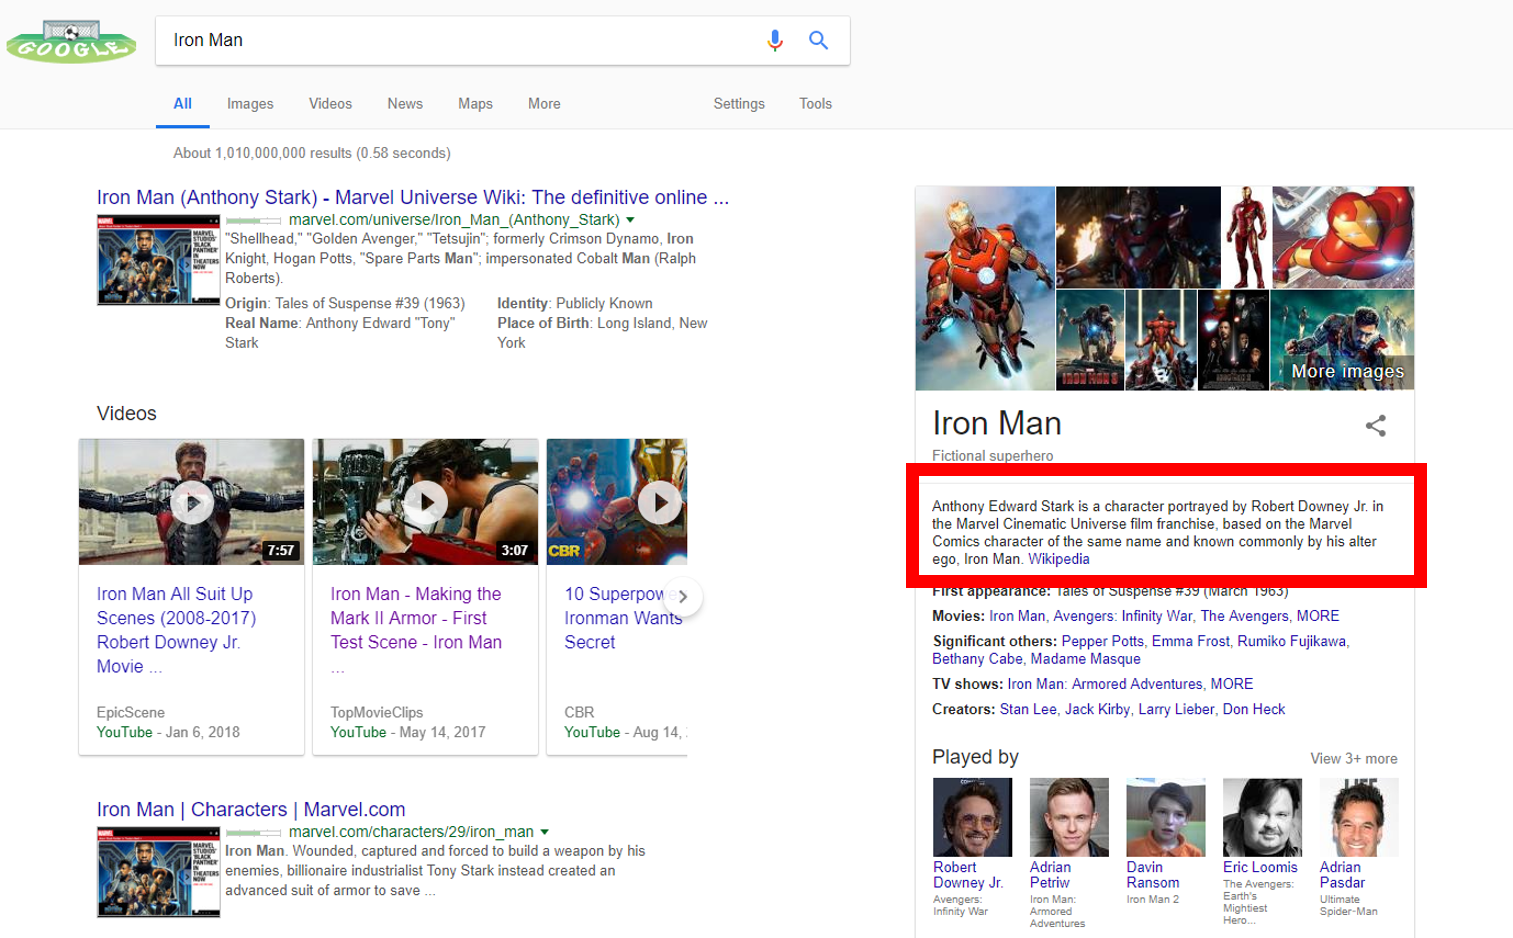
\includegraphics[width=14cm]{figs/ironman.png}
\end{center}
\caption{PC画面でのGoogle Knowledge Panelの表示例}
\label{fig:knowledgepanel}
\end{figure}


\section{システム構成}

本システムは,ある程度知られた知識はGoogleの検索結果にKPが表示されることを利用し,KPの内容を音声によって読み上げる(図\ref{fig:system}).
これにより,ユーザが検索対象情報を得るまでのクリック数を減らすことを目的とする.
言語対応については,英語を対象にしたシステムを想定とする.

音声読み上げについては,text-to-speechに変換を行い,生成された音声を再生する.
使用するアルゴリズムは,自然性の高い読み上げが可能なWaveNet~\cite{Oord2016}を用いる.

生成された音声は,十分に短い時間内で読み上げられる必要がある.
KP内の文章が長すぎる場合には,さらに情報を要約する.
この手法については,\ref{sec:summarize}で詳しく述べる.

\begin{figure}[htb]
\begin{center}
    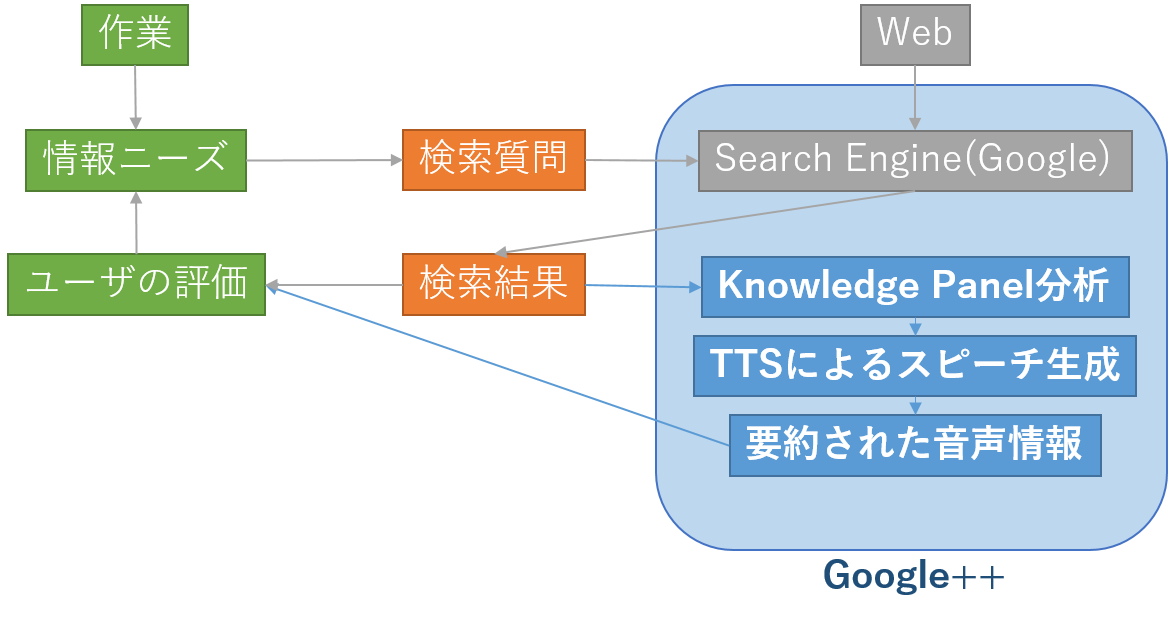
\includegraphics[width=14cm]{figs/system.png}
\end{center}
\caption{}
\label{fig:system}
\end{figure}

\subsection{文章要約手法} \label{sec:summarize}

読み上げ速度は,生成された音声データにより依存する.
これを計測したところ,約$2.3\,\mathrm{words/s}$であった.
情報をユーザに提示する際に,検索結果を確認する時間は,約8秒である~\cite{Granka2004}.
つまり,8秒以内に読み上げる事のできる文章(約$18\,\mathrm{words}$)に要約する.

はじめに参考とする文章は,図\ref{fig:knowledgepanel}における赤枠の部分(knowledge description)を利用する.

\begin{algorithm}
\caption{文章要約アルゴリズム}
\label{alg:summarize}
\begin{algorithmic}
    \STATE $D \leftarrow$ the knowledge description
    \STATE $d \leftarrow D$の最初の文
    \IF{$d$の単語数 $< 18$}
        \RETURN $d$
    \ENDIF

    \STATE $y \Leftarrow 1$
    \IF{$n < 0$}
    \STATE $X \Leftarrow 1 / x$
    \STATE $N \Leftarrow -n$
    \ELSE
    \STATE $X \Leftarrow x$
    \STATE $N \Leftarrow n$
    \ENDIF
    \WHILE{$N \neq 0$}
    \IF{$N$ is even}
    \STATE $X \Leftarrow X \times X$
    \STATE $N \Leftarrow N / 2$
    \ELSE[$N$ is odd]
    \STATE $y \Leftarrow y \times X$
    \STATE $N \Leftarrow N - 1$
    \ENDIF
    \ENDWHILE
\end{algorithmic}
\end{algorithm}




\section{検証実験}

評価項目
\begin{itemize}
    \item 音声だけの情報で満足したか?
    \item 追加の検索したいと考えるか?
    \item 欲しい情報は十分か?
\end{itemize}



\section{結論}


\bibliographystyle{ieee}
\bibliography{references}

\end{document}